\section{Context}
\label{sec:context}

De gebruikers van het systeem zijn onder te verdelen in 5 categori\"{e}n: externen, studenten, professoren, assistenten en programmabeheerders. 
Elk soort gebruiker moet in de finale versie van CalZone in staat zijn de functionaliteiten die specifiek aan deze gebruikers zijn toegekend toe te passen zoals beschreven in het SRS van dit project. 
\\
Gebruikers zijn in staat om zich te registreren in het systeem. 
Hierdoor kunnen ze inloggen en bezitten deze gebruikers een profielpagina.
Daarnaast is de gebruiker in staat deze profielgegevens aan te passen.
In deze iteratie is de functionaliteit voor een algemene gebruiker uitgebreid met de mogelijkheid om lessenroosters en lokalenroosters te bezichtigen.
\\
Eveneens is er functionaliteit voorzien voor specifieke gebruikers: studenten, professoren, assistenten en administrators.
Deze uitbreidingen zijn te bezichtigen in het use case diagram in figuur \ref{fig:usecase}.

\begin{figure}[H]
	\centering
	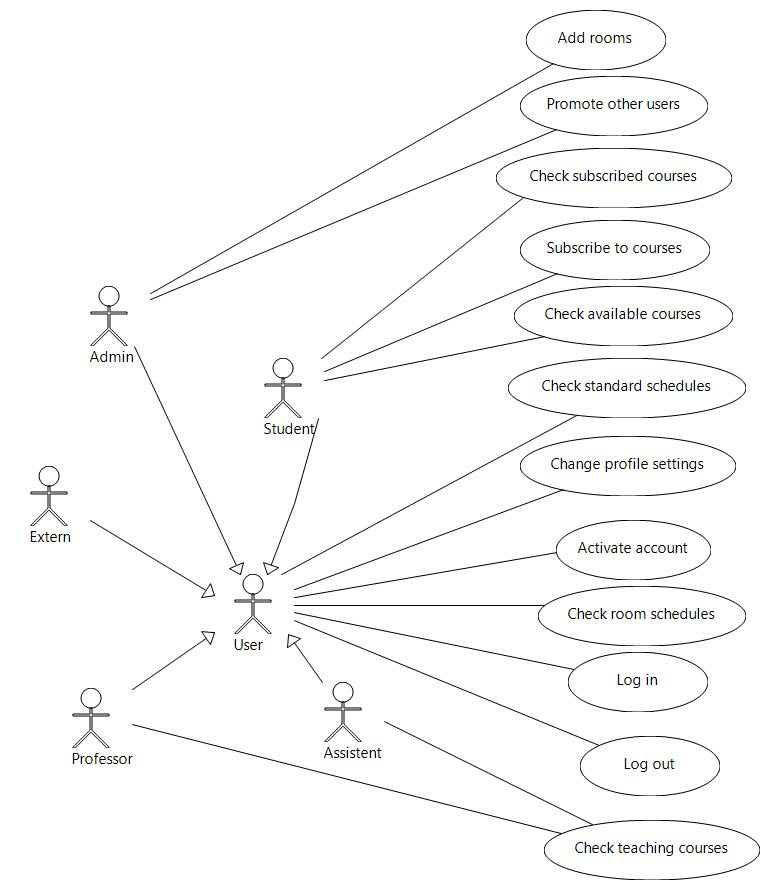
\includegraphics[scale=0.5]{img/use_cases}
	\caption{Use case diagram}
	\label{fig:usecase}
\end{figure}